\subsection{Hotspots}
From the data we gathered, we made several observations that benefits the features to be included in the model we present. We separate the data into different time frames in order to determine the overall difference among them, since charging network is a dynamic system.
\begin{figure}[htbp]
	\begin{tabular}{cc}
		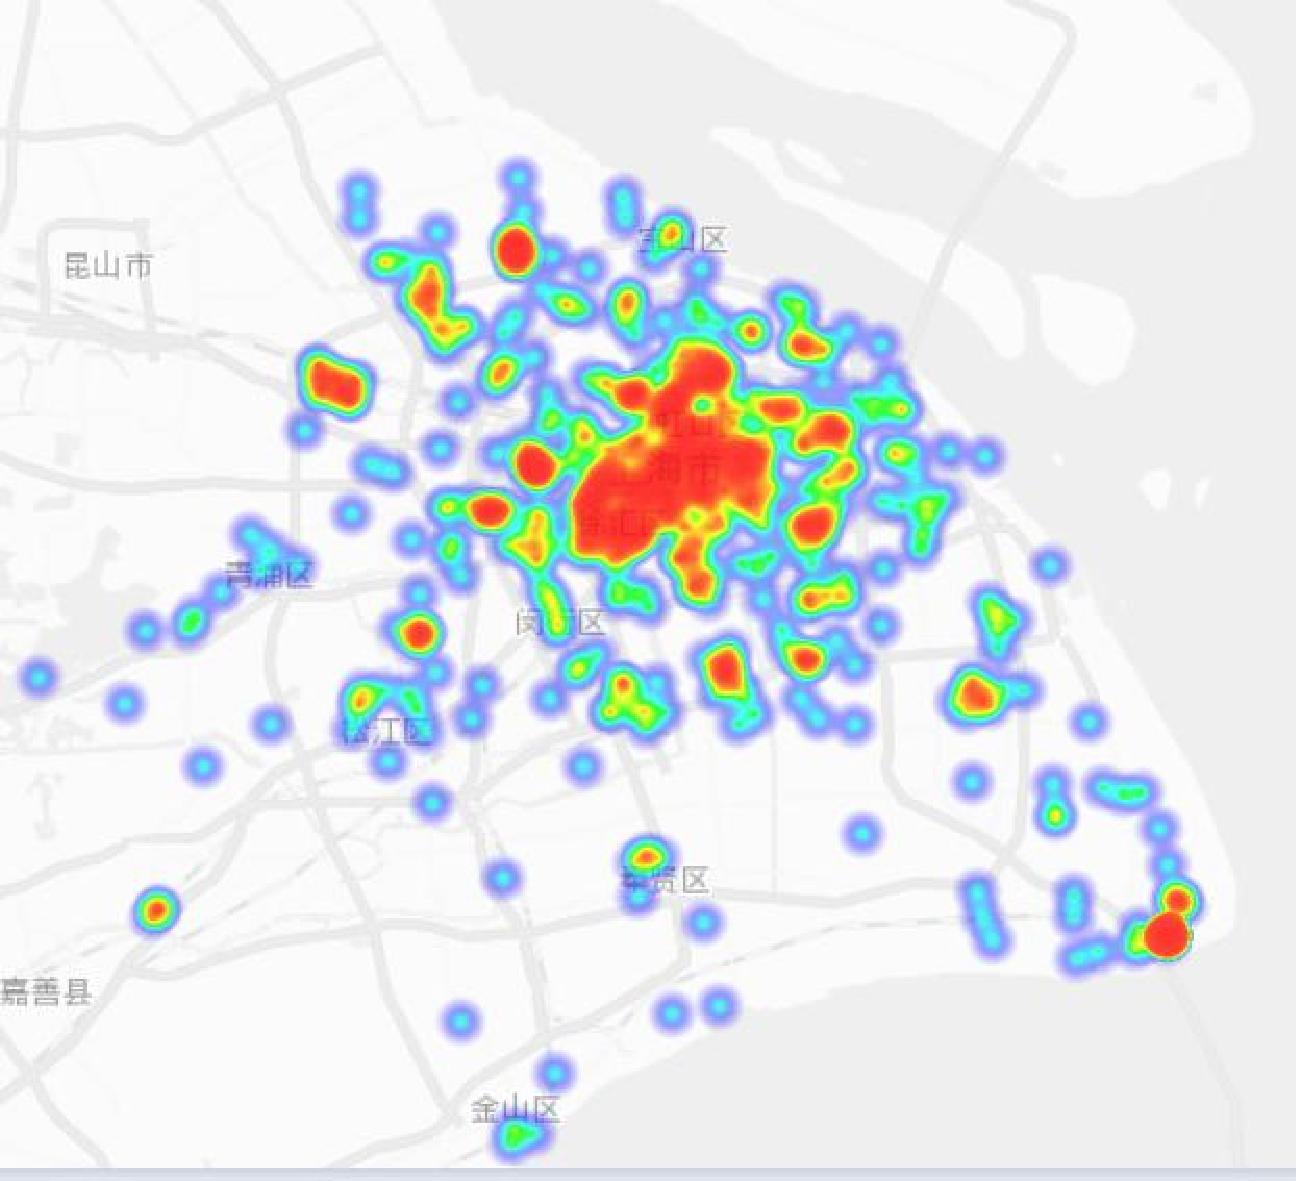
\includegraphics[width=0.45\columnwidth]{./figures/weekday.pdf} &  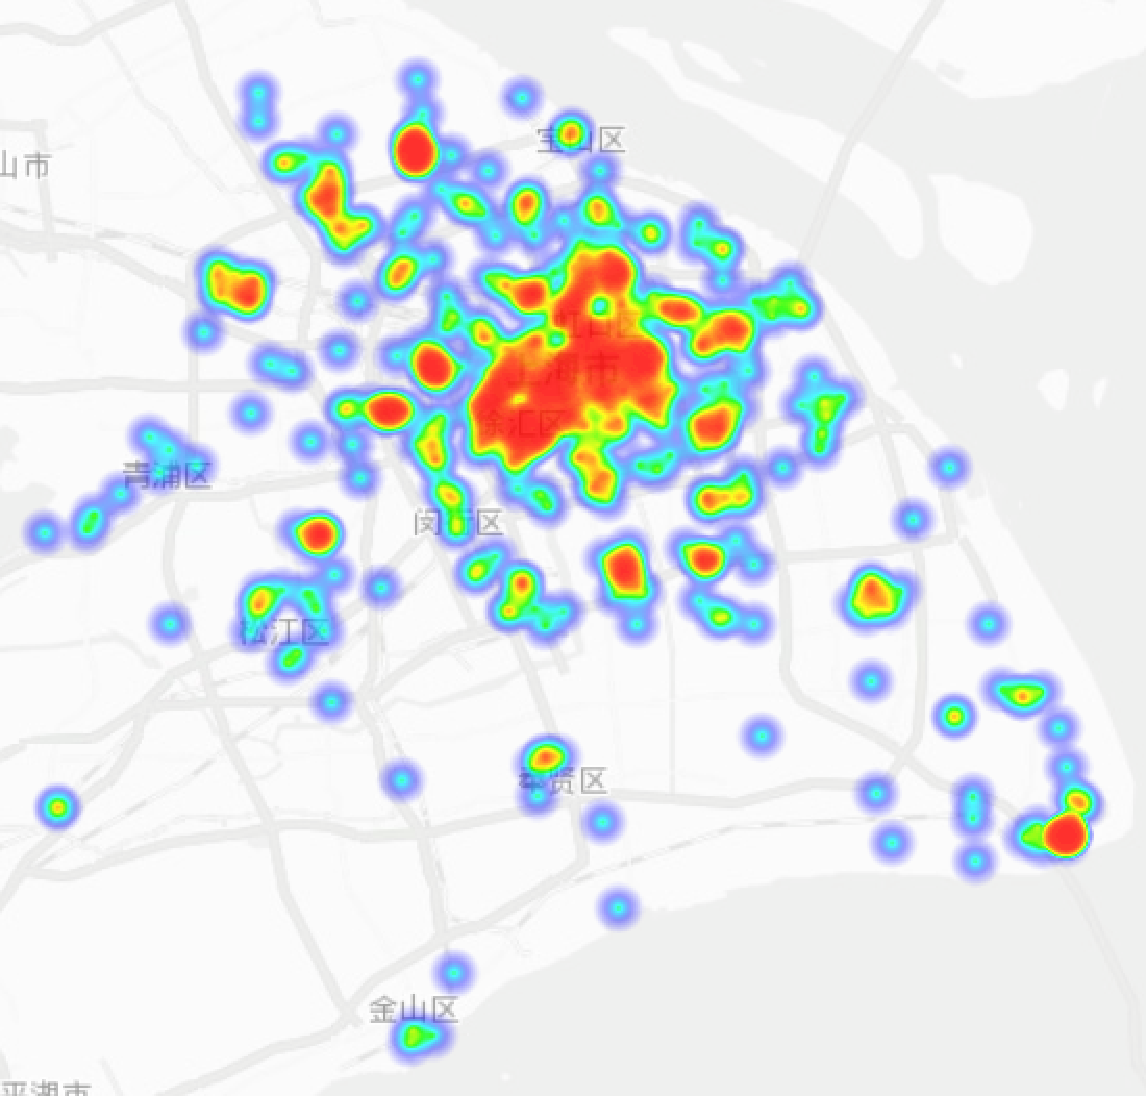
\includegraphics[width=0.45\columnwidth]{./figures/weekend.pdf} \\
		(a) Weekdays & (b) Weekends \\[6pt] 
		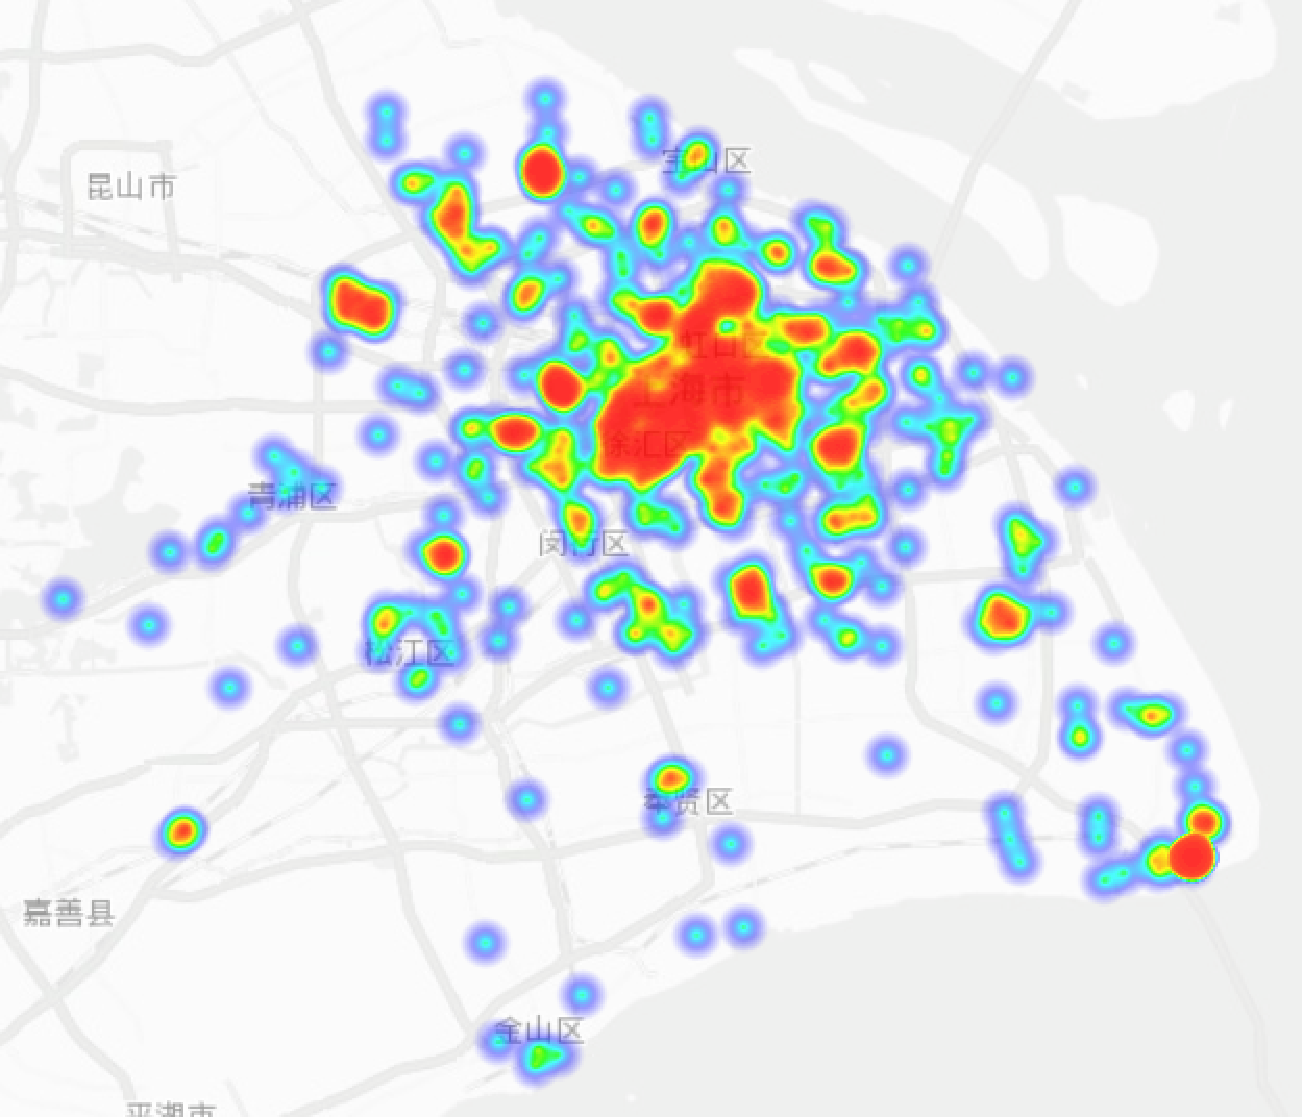
\includegraphics[width=0.45\columnwidth]{./figures/morning.pdf} &
		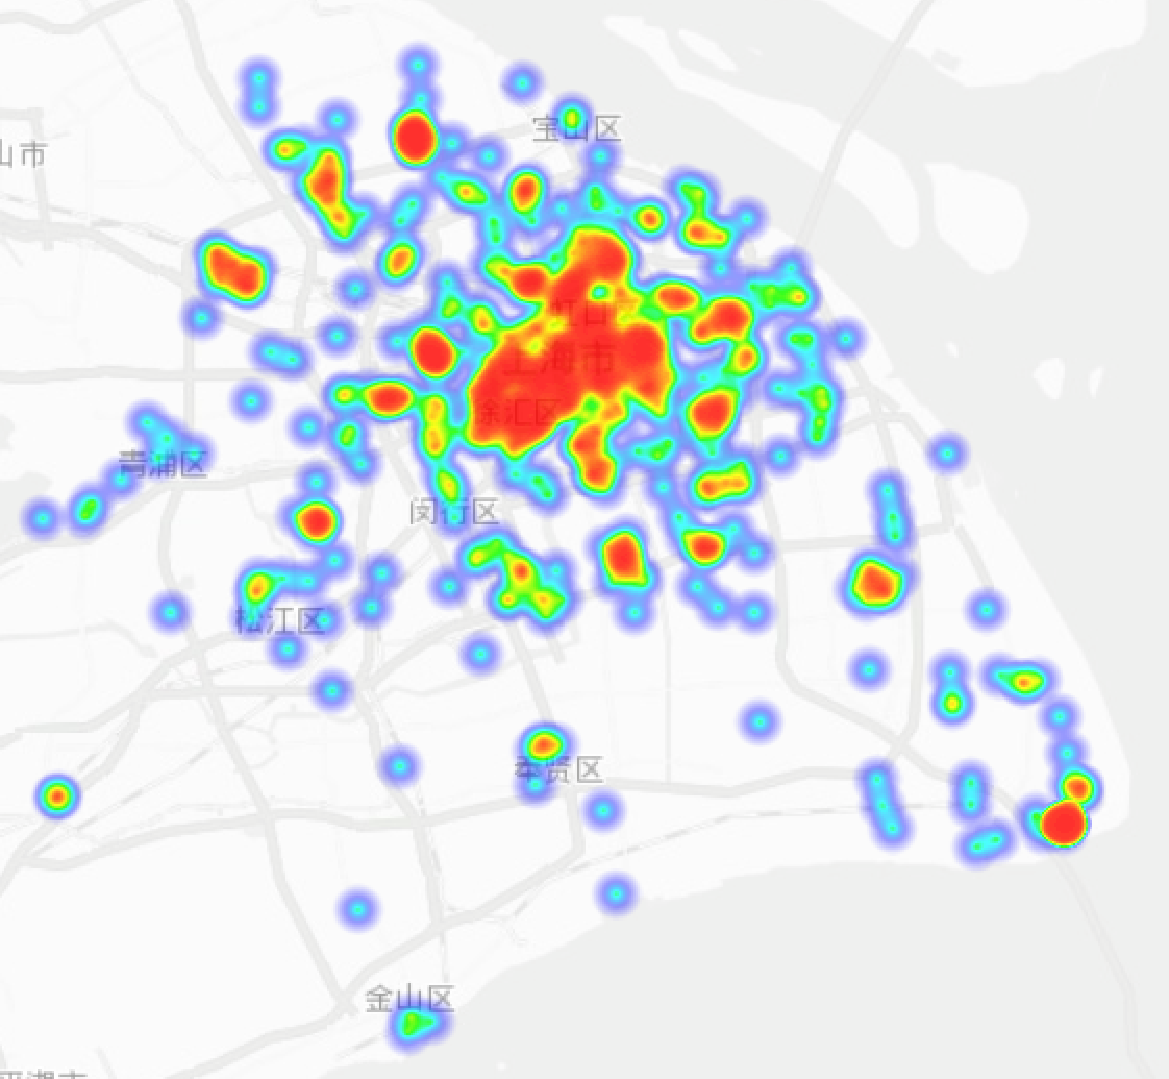
\includegraphics[width=0.45\columnwidth]{./figures/evening.pdf} \\
		(c) Mornings & (d) Evenings
	\end{tabular}
	\centering
	\caption{Charging Hotspots in Shanghai in different time frames}
	\label{fig2}
\end{figure}
From Fig.\ref{fig2}, it is easy to notice that in different time frames, the charging hotspots stays at almost the same locations, meaning that during different time periods, the use rate of a given charging station is determined by its spatiotemporal context.

\subsection{Point Of Interest}
To the prosperity of Shanghai, there are so many points of interest(e.g., shopping malls, schools. estates, companies, etc.) located in the city.  Understanding the purpose of the trip by each person who participates in charging system will help us to analyze the use rate prediction. So, we need to extract the POI around each existing charging station. There are a lot of POIs in Shanghai. The POIs are very close to each other. We set a radius around each station and then collect the POIs within the radius. Based on our experiment, choosing a radius as 300 meters is proper. In our work, we get 80 different types of POI totally. Some of the POIs are very similar to each other. Therefore, we group 80 POIs in further step. By grouping POIs, we get 10 groups at last. Table.\ref{tab1} gives the groups and POIs in detail.

\begin{table}[htbp]
	\caption{Groups of POIs}
	\begin{center}
		\begin{tabular}{|l|p{5cm}|}
			\hline
			Group & Points of interests\\
			\hline
			Food & chinese \& foreign restaurant, snack bar, cake \& dessert shop, cafe, bar\\
			\hline
			Hotels & star hotel, express hotel, apartment hotel\\
			\hline
			Shopping & shopping centers, department stores, supermarkets, convenience stores, home building materials, home appliances digital, shops, markets\\
			\hline
			Education & institutions of higher learning, middle schools, primary schools, kindergartens, adult education, parent-child education, special education schools, study agencies, research institutions, training institutions, libraries, science and technology museums\\
			\hline
			Cultural venue & press and publication, radio and television, art groups, art galleries, exhibition halls, cultural palaces\\
			\hline
			Medical & general hospitals, specialist hospitals, clinics, pharmacies, medical examination institutions, nursing homes, emergency centers, disease control centers\\
			\hline
			Car service & car sales, car repair, car beauty, auto parts, car rental, car inspection field\\
			\hline
			Transportation & airport, railway station, subway station, subway line, long-distance bus station, bus station, bus line, port, parking lot, refueling station, service area, toll station, bridge, charging station, roadside parking space\\
			\hline
			Estates & Office building, residential area, dormitory\\
			\hline
		\end{tabular}
		\label{tab1}
	\end{center}
\end{table}

\subsection{Distance}

In use rate prediction, we need to consider distance. People will not choose to park their electric cars for charging if the destination they planned to go is far away. In the system, a station with nearer distance to metro stations, financial centers and major functional buildings would easily be used more often. We select the nearest distance to the following to be the distance we considered as features: company, estate, hospital, metro station, shopping center and university.

\subsection{Price}
By futher digging into the data, we find that there is a 0.3 correlation between price for charging and the use rate. Since there are two types of charging ports: DC and AC. We would include the number of ports and the price of both types in a charging station as one of its feature.

\subsection{Private or public}
By observing the data we've collected, it can be seen that most of the charging stations are private charging stations, which means they are typically used by electric public buses and rent cars, or used by specific companies for their employees, accounting for over 70\% of the total charging stations. Also, since the private are used by more regular users(e.g., buses, companies employees), its use rate are 5\% higher compared to public ones. This alongside other observations will be taken into consideration.
